\documentclass[a4paper]{article}
\usepackage[pdftex]{hyperref}
\usepackage[latin1]{inputenc}
\usepackage[english]{babel}
\usepackage{a4wide}
\usepackage{amsmath}
\usepackage{amssymb}
\usepackage{algorithmic}
\usepackage{algorithm}
\usepackage{ifthen}
\usepackage{listings}
% move the asterisk at the right position
\lstset{basicstyle=\ttfamily,tabsize=4,literate={*}{${}^*{}$}1}
%\lstset{language=C,basicstyle=\ttfamily}
\usepackage{moreverb}
\usepackage{palatino}
\usepackage{multicol}
\usepackage{tabularx}
\usepackage{comment}
\usepackage{verbatim}
\usepackage{color}

%% pdflatex?
\newif\ifpdf
\ifx\pdfoutput\undefined
\pdffalse % we are not running PDFLaTeX
\else
\pdfoutput=1 % we are running PDFLaTeX
\pdftrue
\fi
\ifpdf
\usepackage[pdftex]{graphicx}
\else
\usepackage{graphicx}
\fi
\ifpdf
\DeclareGraphicsExtensions{.pdf, .jpg}
\else
\DeclareGraphicsExtensions{.eps, .jpg}
\fi

\parindent=0cm
\parskip=0cm

\setlength{\columnseprule}{0.4pt}
\addtolength{\columnsep}{2pt}

\addtolength{\textheight}{5.5cm}
\addtolength{\topmargin}{-26mm}
\pagestyle{empty}

%%
%% Sheet setup
%% 
\newcommand{\coursename}{Image Processing}
\newcommand{\courseno}{CAS-320321}
 
\newcommand{\sheettitle}{Homework}
\newcommand{\mytitle}{}
\newcommand{\mytoday}{{February 20}, 2020}

% Current Assignment number
\newcounter{assignmentno}
\setcounter{assignmentno}{1}

% Current Problem number, should always start at 1
\newcounter{problemno}
\setcounter{problemno}{1}

%%
%% problem and bonus environment
%%
\newcounter{probcalc}
\newcommand{\problem}[2]{
  \pagebreak[2]
  \setcounter{probcalc}{#2}
  ~\\
  {\large \textbf{Problem {\arabic{assignmentno}}.{\arabic{problemno}}} \hspace{0.2cm}\textit{#1}} \refstepcounter{problemno}\vspace{2pt}\\}

\newcommand{\bonus}[2]{
  \pagebreak[2]
  \setcounter{probcalc}{#2}
  ~\\
  {\large \textbf{Bonus Problem {\arabic{assignmentno}}.{\arabic{problemno}}} \hspace{0.2cm}\textit{#1}} \refstepcounter{problemno}\vspace{2pt}\\}

%% some counters  
\newcommand{\assignment}{\arabic{assignmentno}}

%% solution  
\newcommand{\solution}{\pagebreak[2]{\bf Solution:}\\}

%% Hyperref Setup
\hypersetup{pdftitle={Homework \assignment},
  pdfsubject={\coursename},
  pdfauthor={},
  pdfcreator={},
  pdfkeywords={Computer Architecture and Programming Languages},
  %  pdfpagemode={FullScreen},
  %colorlinks=true,
  %bookmarks=true,
  %hyperindex=true,
  bookmarksopen=false,
  bookmarksnumbered=true,
  breaklinks=true,
  %urlcolor=darkblue
  urlbordercolor={0 0 0.7}
}

\begin{document}
\coursename \hfill Course: \courseno\\
Jacobs University Bremen \hfill \mytoday\\
{Otmane Sabir}\hfill \\
{Aadil Anil Kumar}\hfill
\vspace*{0.3cm}\\
\begin{center}
{\Large \sheettitle{} {\assignment}\\}
\end{center}
\\

\large\texbf{Experiment 1: Symmetric (SE5.txt) vs. Asymmetric (SE7.txt) SE} \\

\begin{figure}[ht] 
  \label{ fig7} 
  \begin{minipage}[b]{0.5\linewidth}
    \centering
    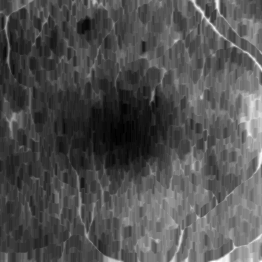
\includegraphics[width=.95\linewidth]{eroSym.png} 
    \caption{Erosion with Symmetric SE} 
    \vspace{4ex}
  \end{minipage}%%
  \begin{minipage}[b]{0.5\linewidth}
    \centering
    \includegraphics[width=.95\linewidth]{eroAsym.png} 
    \caption{Erosion with Asymmetric SE} 
    \vspace{4ex}
  \end{minipage} 
  \begin{minipage}[b]{0.5\linewidth}
    \centering
    
\includegraphics[width=.95\linewidth]{closSym.jpg} 
    \caption{Closing with Symmetric SE} 
    \vspace{4ex}
  \end{minipage}%% 
  \begin{minipage}[b]{0.5\linewidth}
    \centering
    
\includegraphics[width=.95\linewidth]{closAsym.jpg} 
    \caption{Closing with Asymmetric SE} 
    \vspace{4ex}
  \end{minipage} 
\end{figure} \\
Border effects tend to occur when using an asymmetric SE that does not fit the definition domain of the image set.
As expected the chosen border handling method does introduce artifacts to the image.\\ \\
A possible explanation for this could be the fact that the definition domain of the image set decreases when doing the operation due to image borders not being handled correctly.\\ \\
If you were to observe and compare Figure 1 and 2 closely you can see that the bottom border of Figure 2 contains a row of white space. This is evident when viewing the image with a black background. The effects were more pronounced when doing a comparison of the closing operation, as shown in figure 3 and 4.

\newpage
\large\texbf{Experiment 2: Improving the clarity of handwritten digits} \\ 

Problem: Classification of handwritten digits \\
\begin{figure}[htp]
    \centering
    
\includegraphics[width=8cm]{six.png}
    \caption{Original image, res: 602\times599}
    \label{fig:erosionSym}
\end{figure}\\
As visible in the image above, the six is a little thick with the white circle in the middle not that evident.
\begin{figure}[htp]
    \centering
    
\includegraphics[width=8cm]{dilated_six.png}
    \caption{Dilated six}
    \label{fig:erosionAsym}
\end{figure}\\
After dilating the image with a structuring element that is a square of size 15 (SE10.txt), we get a sharper six.\\

We chose this structuring element because we saw that the six was formed using square blots. We decided to use a larger structuring element because the image is very pixelated and we wanted to see a clear circle in the center of the six.\\

A possible use case for this would be feature extraction. A classification algorithm could more efficiently extract features that maps the digit as a six.

\newpage
\large\texbf{Experiment 3: Cell segmentation} \\

Problem: Clear segmentation of the cells in order to assist with counting.\\
\begin{figure}[htp]
    \centering
    \includegraphics[width=7.5cm]{nuclei.png}
    \caption{Original image, res: 1344\times1024}
    \label{fig:erosionSym}
\end{figure}
\begin{figure}[ht] 
  \label{ fig7} 
  \begin{minipage}[b]{0.5\linewidth}
    \centering
    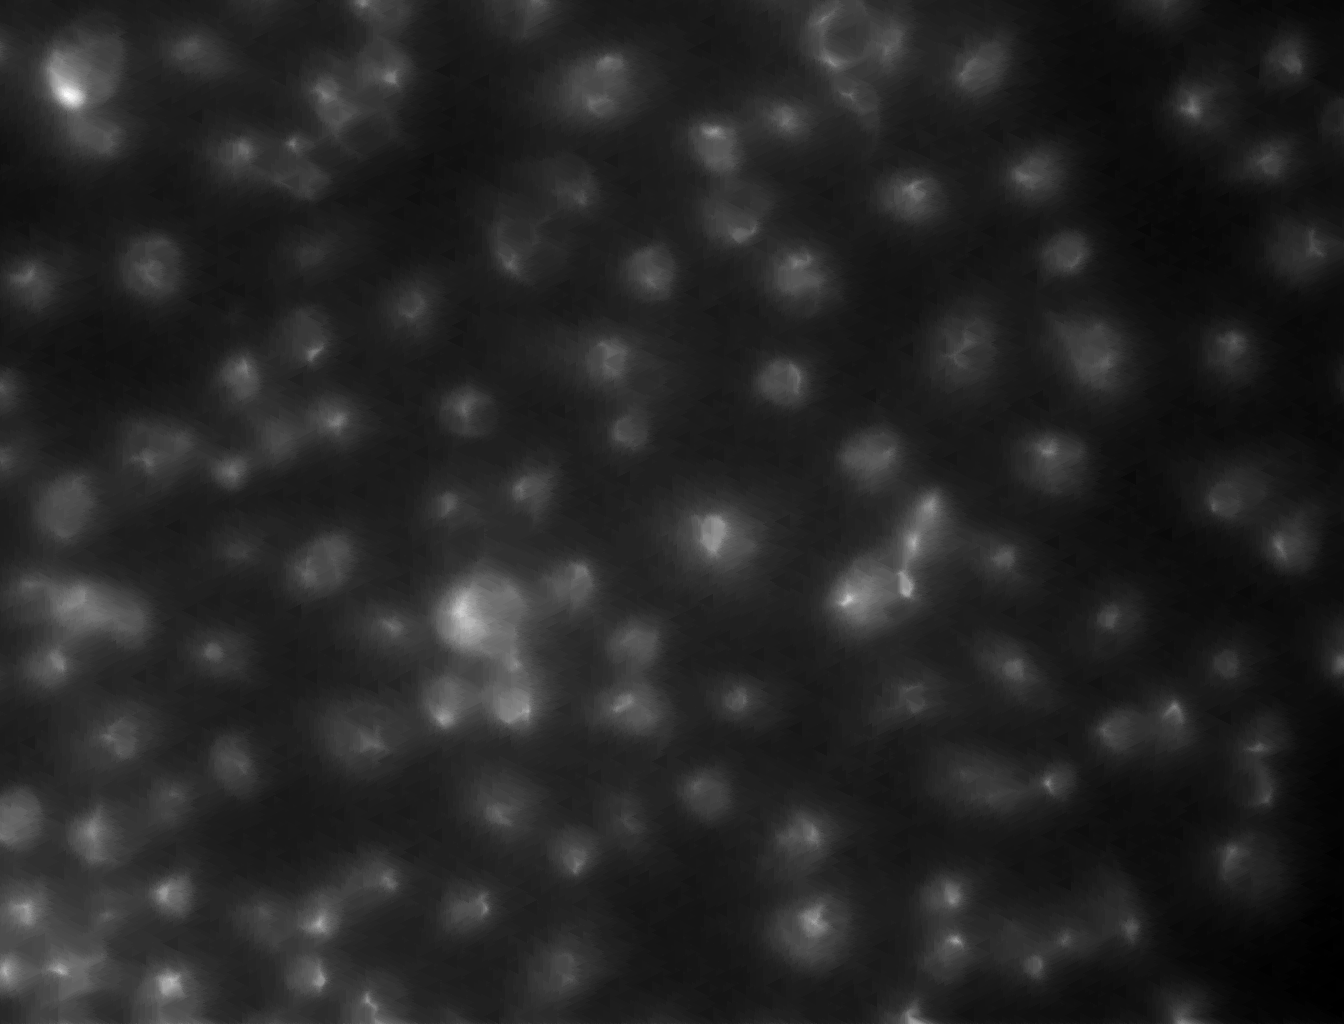
\includegraphics[width=.95\linewidth]{nuclei_erosion.png} 
    \caption{Erosion} 
    \vspace{4ex}
  \end{minipage}%%
  \begin{minipage}[b]{0.5\linewidth}
    \centering
    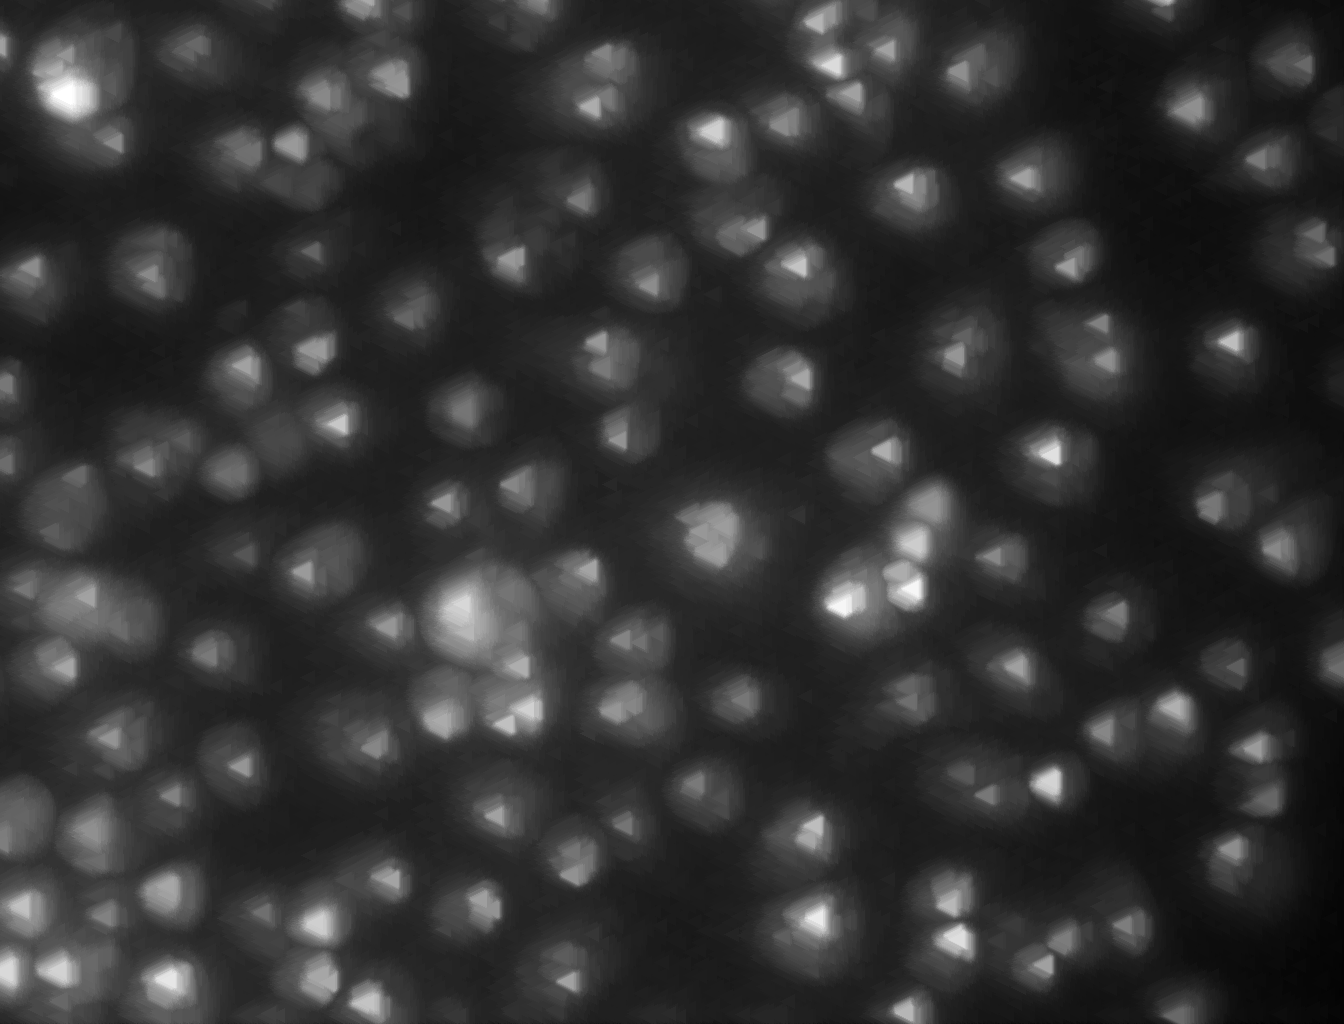
\includegraphics[width=.95\linewidth]{nuclei_dilation.png} 
    \caption{Dilation} 
    \vspace{4ex}
  \end{minipage} 
  \begin{minipage}[b]{0.5\linewidth}
    \centering
    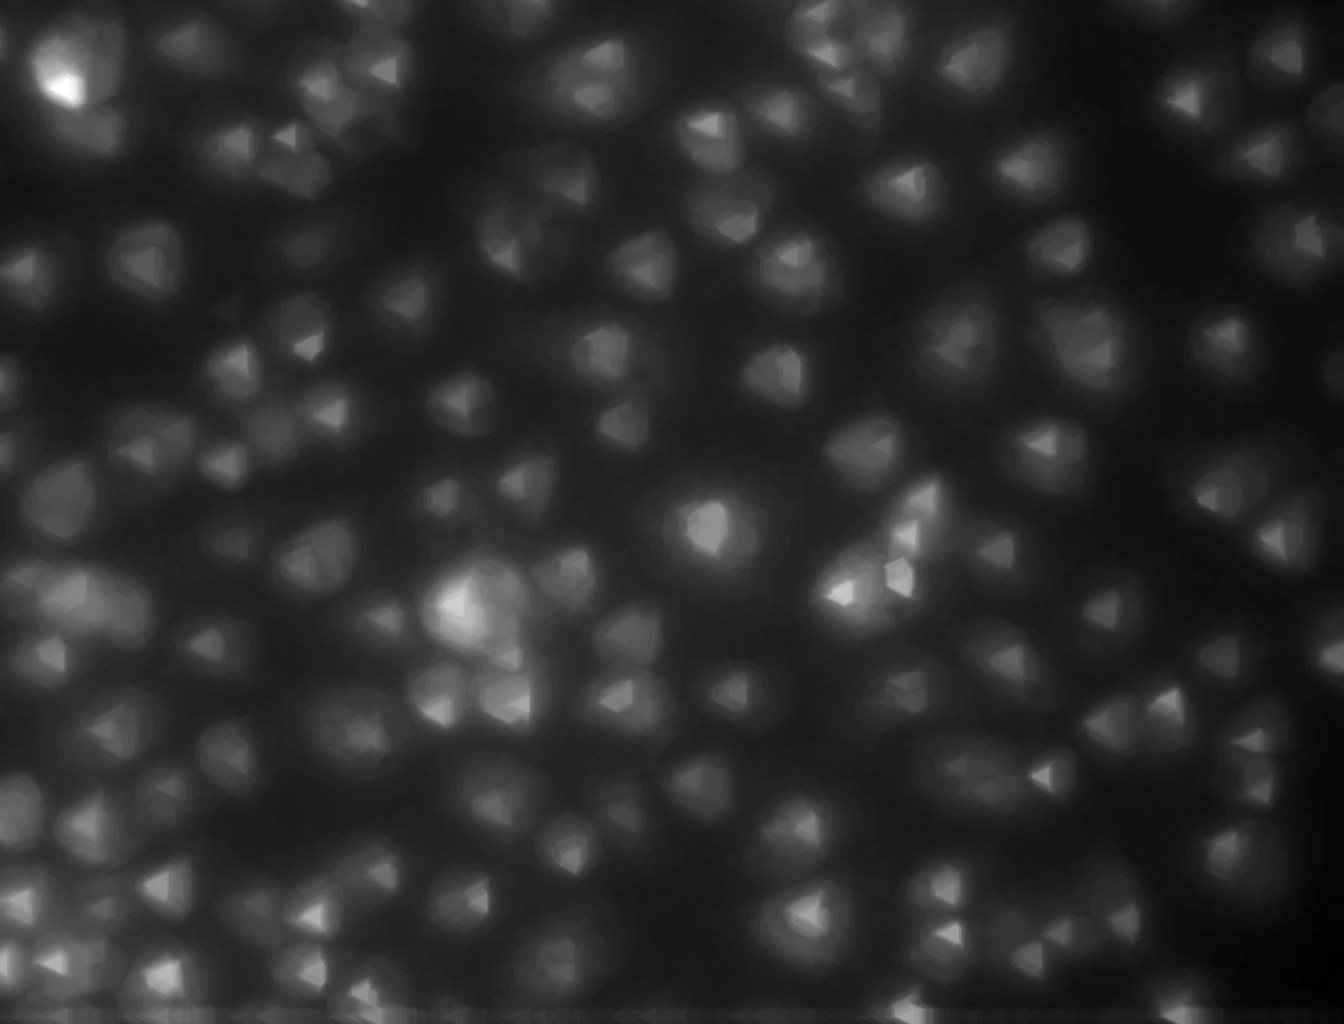
\includegraphics[width=.95\linewidth]{opening.png} 
    \caption{Opening} 
    \vspace{4ex}
  \end{minipage}%% 
  \begin{minipage}[b]{0.5\linewidth}
    \centering
    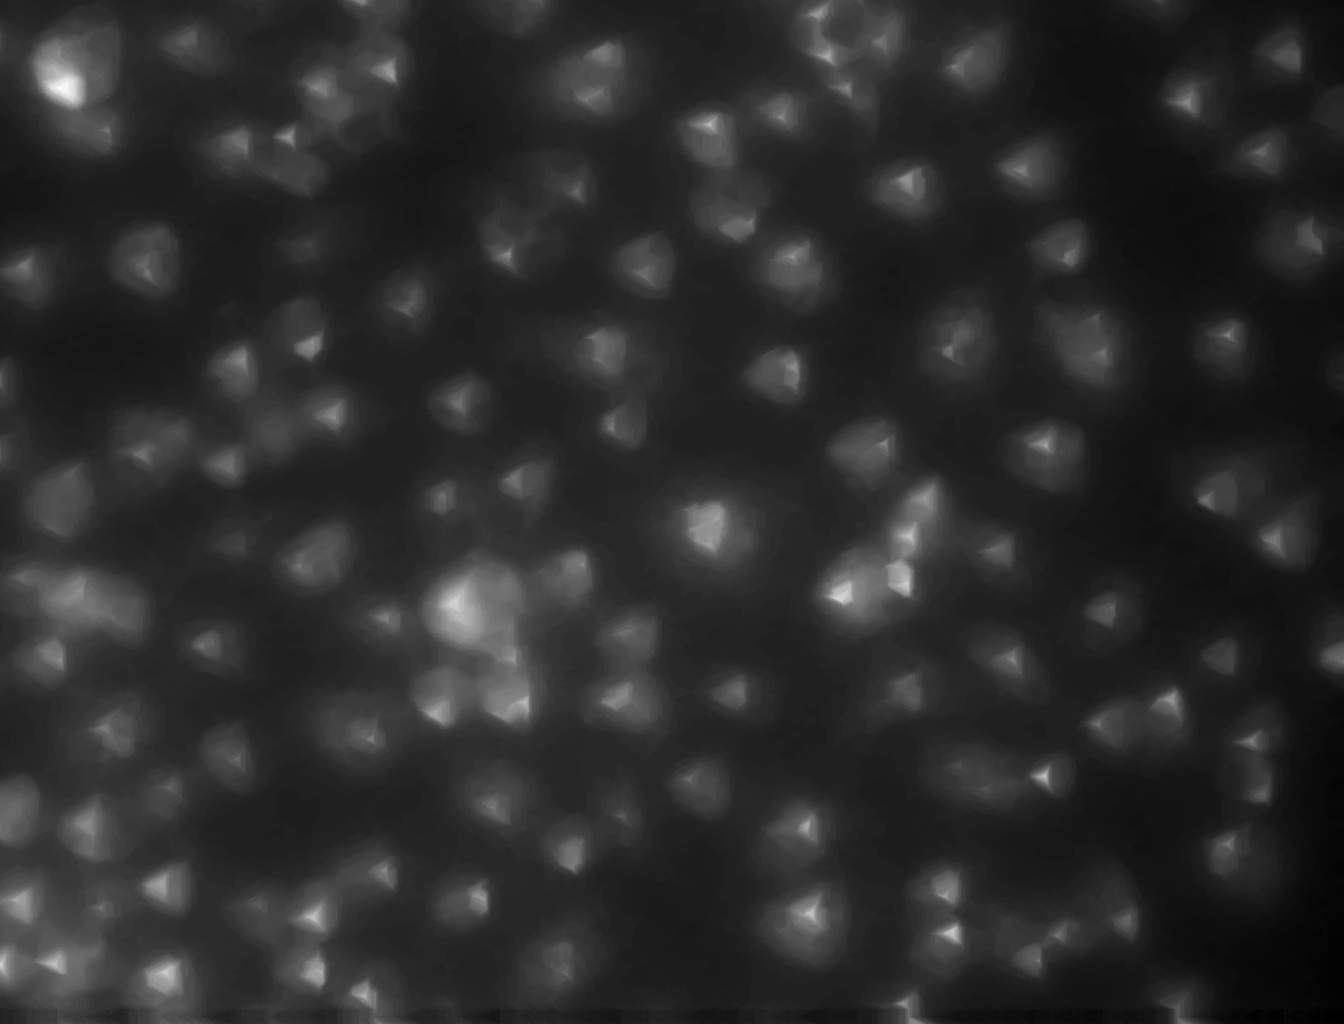
\includegraphics[width=.95\linewidth]{nuclei_closing.png} 
    \caption{Closing} 
    \vspace{4ex}
  \end{minipage} 
\end{figure} 

For these operations we used a parallelogram structuring element(SE11). We chose this shape for this image as there are a lot of circular structures that we wanted to highlight. There is a lot more contrast in the images that had the operations done on them; helping clearly segment each cellular structure.\\

The dilated image has the clearest segmentation between structures. However, the opened image also shows clear segmentation while not having as jarring of a contrast. \\


\large{Experiment 4: Haemoglobin noise filtering and cell filling} \\

Problem: Count of the amount of red blood cells in the blood smear image.
\begin{figure}[htp]
    \centering
    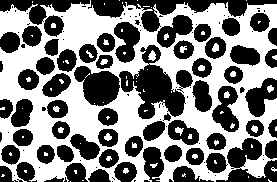
\includegraphics[width=8cm]{redblood.png}
    \caption{Original image, res: 277\times182}
    \label{fig:erosionSym}
\end{figure}\\

In order to assist in the counting of the red blood cells present in this image, we would first remove the evident noise then proceed to fill in the holes in the middle of the cells as best as possible. 
\\
\begin{figure}[ht] 
  \label{ fig7} 
  \begin{minipage}[b]{0.5\linewidth}
    \centering
    \includegraphics[width=.97\linewidth]{c_redbloodse4.png} 
    \caption{Closing with SE4} 
    \vspace{4ex}
  \end{minipage}%%
  \begin{minipage}[b]{0.5\linewidth}
    \centering
    \includegraphics[width=.97\linewidth]{e_closedredbloodse3.png} 
    \caption{Erosion of closed image with SE3} 
    \vspace{4ex}
  \end{minipage} 
\end{figure} 

We decided to perform a closing operation to remove the small black spots present then fill in some of the white spaces present in the cell. After comparing the results of a size 3 and size 4 square, we found that the latter worked better in removing the noisy elements within this picture. \\

Performing the closing led to the red blood cells not being as defined. In order to fill in the holes and accentuate the features of the cells we decided to perform a erosion on the closed image using a vertical SE of length 3. \\

However, additional operations would need to be done in order to further fill in the center of some of the cells. 

\newpage

\large{Experiment 5: Fingerprint image cleaning} \\

Problem: Removal of the noise present in this image and sharpen the image further to create a clearer fingerprint.\\

\begin{figure}[htp]
    \centering
    \includegraphics[height=8cm]{fingerprint.png}
    \caption{Original image, res:332\times450}
    \label{fig:erosionSym}
\end{figure}\\

\\
\begin{figure}[ht] 
  \label{ fig7} 
  \begin{minipage}[b]{0.5\linewidth}
    \centering
    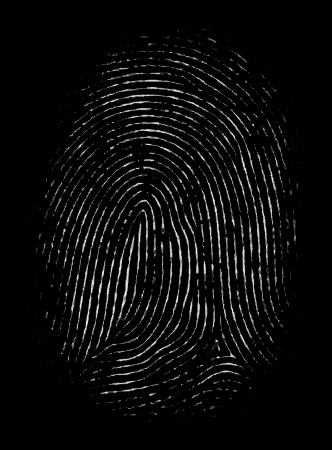
\includegraphics[height=.97\linewidth]{e_fingerprint.png} 
    \caption{Closing with SE4} 
    \vspace{4ex}
  \end{minipage}%%
  \begin{minipage}[b]{0.5\linewidth}
    \centering
    \includegraphics[height=.97\linewidth]{o_fingerprint.png} 
    \caption{Erosion of closed image with SE3} 
    \vspace{4ex}
  \end{minipage} 
\end{figure} 

There are quite a few white spots surrounding the fingerprint. This led us to using a square of size 3 (SE1.txt) in order to remove these spots.\\

After performing an erosion we get an image without the white squares, however it also leads to a darker fingerprint.\\

In order to further define the print lines decided to perform and opening function which produces a far better result. Giving us a clear and defined fingerprint.

\end{document}
